\documentclass[letterpaper, 12pt]{math}

\usepackage{tikz}

\title{University Physics 1A}
\author{Alvin Lin}
\date{September 14th, 2017}

\begin{document}

\maketitle

\section*{Circular Motion}
\begin{center}
  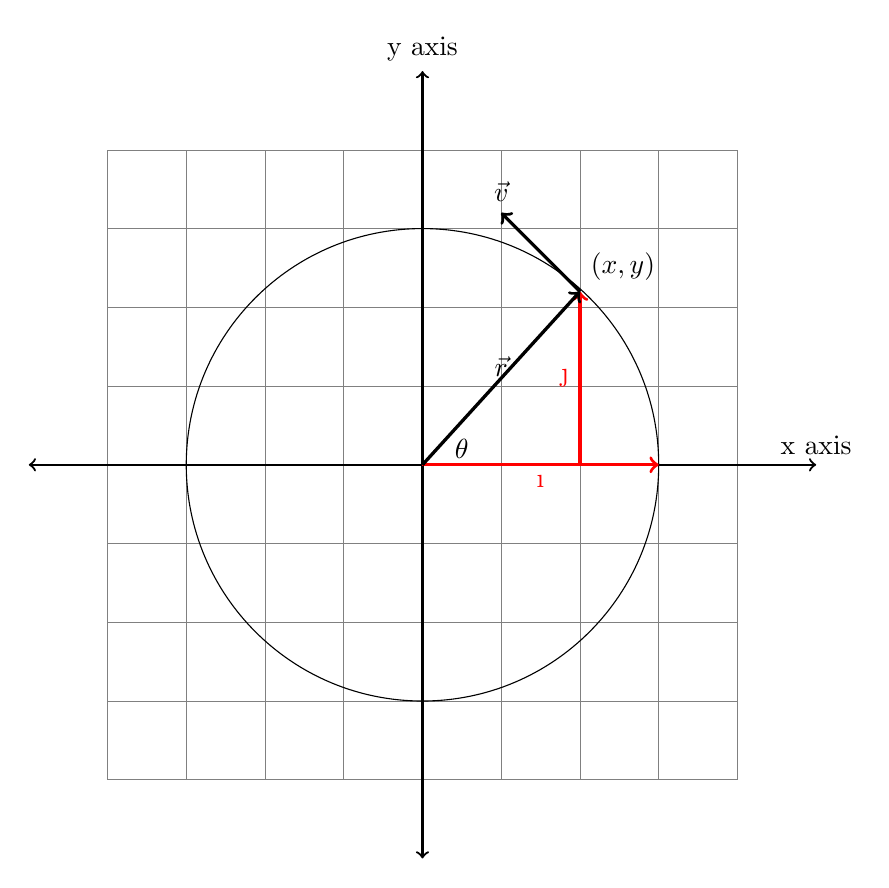
\begin{tikzpicture}
    \draw[step=1cm,gray,very thin] (-4,-4) grid (4,4);
    \draw[thick,<->] (-5,0) -- (5,0) node[above] {x axis};
    \draw[thick,<->] (0,-5) -- (0,5) node[above] {y axis};
    \draw (0,0) circle (3cm);
    \draw[very thick,red,->] (0,0) -- (3,0) node[pos=0.5, below] {\( \i \)};
    \draw[very thick,red,->] (2,0) -- (2,2.2) node[pos=0.5, left] {\( \j \)};
    \draw[very thick,->] (0,0) -- (2,2.2) node[above right] {\( (x,y) \)};
    \draw[very thick,->] (2,2.2) -- (1,3.2) node[above] {\( \vec{v} \)};
    \node[above] (A) at (1,1) {\( \vec{r} \)};
    \node (B) at (0.5,0.2) {\( \theta \)};
  \end{tikzpicture}
\end{center}
The position of an object in circular motion:
\[ \vec{r} = x\i+y\j \]

\subsubsection*{Constant Speed}
\begin{align*}
  \text{speed } v &= \frac{\text{distance traveled}}{\text{time}} \\
  &= \frac{\text{arc length}}{\text{time}} \\
  &= \frac{r\theta}{t}
\end{align*}
where \( t \) is the time it takes to travel \( \theta \).
\begin{align*}
  \theta &= \frac{vt}{r} \\
  \vec{r} &= x\i+y\j \\
  &= r\cos\theta\i+r\sin\theta\j \\
  \vec{r} &= r\cos(\frac{vt}{r})\i+r\sin(\frac{vt}{r})\j \\
  \vec{v} &= \ddiff{\vec{r}}{t} \\
  &= -r\frac{v}{r}\sin(\frac{vt}{r})+r\frac{v}{r}\cos(\frac{vt}{r})\j \\
  &= -v\sin(\frac{vt}{r})\i+v\cos(\frac{vt}{r})\j \\
  \vec{a} &= \ddiff{\vec{v}}{t} \\
  &= -v\frac{v}{r}\cos(\frac{vt}{r})\i-v\frac{v}{r}\sin(\frac{vt}{r})\j \\
  &= -\frac{v^2}{r}(\cos(\frac{vt}{r})\i+\sin(\frac{vt}{r})\j) \\
  \|\vec{a}\| &= \frac{v^2}{r} \\
\end{align*}
Note that the direction of \( \vec{a} \) is the opposite of \( \vec{r} \) and
points towards the center of the circle.

\subsubsection*{Changing Speed}
If \( v\) is not constant:
\begin{center}
  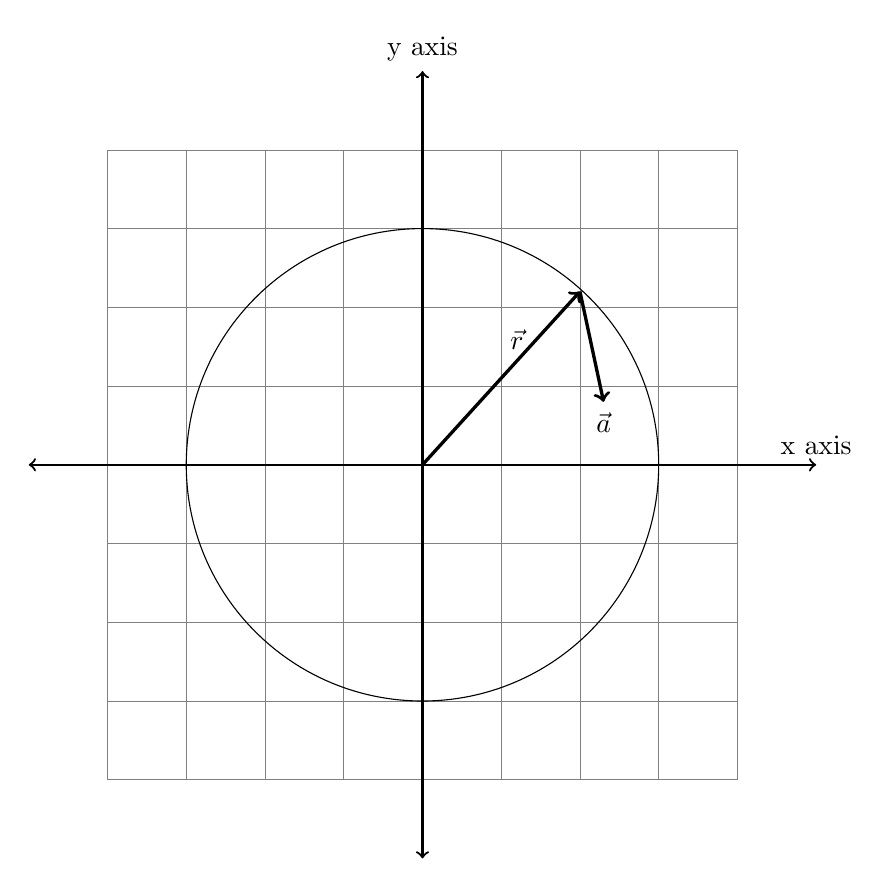
\begin{tikzpicture}
    \draw[step=1cm,gray,very thin] (-4,-4) grid (4,4);
    \draw[thick,<->] (-5,0) -- (5,0) node[above] {x axis};
    \draw[thick,<->] (0,-5) -- (0,5) node[above] {y axis};
    \draw (0,0) circle (3cm);
    \draw[very thick,->] (0,0) -- (2,2.2) node[pos=0.6,above] {\( \vec{r} \)};
    \draw[very thick,->] (2,2.2) -- (2.3,0.8) node[below] {\( \vec{a} \)};
  \end{tikzpicture}
\end{center}
\begin{center}
  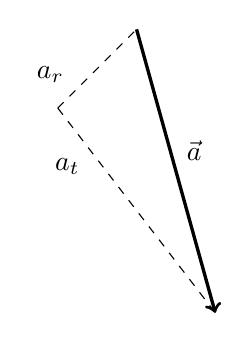
\begin{tikzpicture}
    \draw[very thick,->] (1,1) -- (2,-2.6) node[pos=0.5,above right]
      {\( \vec{a} \)};
    \draw[dashed] (0,0) -- (1,1) node[pos=0.2, above left] {\( a_r \)};
    \draw[dashed] (0,0) -- (2,-2.6) node[pos=0.2, below left] {\( a_t \)};
  \end{tikzpicture}
\end{center}
\begin{align*}
  a_r &= \frac{v^2}{r} \\
  a_t &= \ddiff{v}{t} = \text{rate of change of speed}
\end{align*}

\section*{Reminders and Homework}
Complete the homework on TheExpertTA and WebAssign. \\
\textbf{Remember to bring the Activities Manual}

\begin{center}
  You can find all my notes at \url{http://omgimanerd.tech/notes}. If you have
  any questions, comments, or concerns, please contact me at
  alvin@omgimanerd.tech
\end{center}

\end{document}
